\documentclass{sigchi}

% Use this command to override the default ACM copyright statement
% (e.g. for preprints).  Consult the conference website for the
% camera-ready copyright statement.

%% EXAMPLE BEGIN -- HOW TO OVERRIDE THE DEFAULT COPYRIGHT STRIP -- (July 22, 2013 - Paul Baumann)
% \toappear{Permission to make digital or hard copies of all or part of this work for personal or classroom use is      granted without fee provided that copies are not made or distributed for profit or commercial advantage and that copies bear this notice and the full citation on the first page. Copyrights for components of this work owned by others than ACM must be honored. Abstracting with credit is permitted. To copy otherwise, or republish, to post on servers or to redistribute to lists, requires prior specific permission and/or a fee. Request permissions from permissions@acm.org. \\
% {\emph{CHI'14}}, April 26--May 1, 2014, Toronto, Canada. \\
% Copyright \copyright~2014 ACM ISBN/14/04...\$15.00. \\
% DOI string from ACM form confirmation}
%% EXAMPLE END -- HOW TO OVERRIDE THE DEFAULT COPYRIGHT STRIP -- (July 22, 2013 - Paul Baumann)

% Arabic page numbers for submission.  Remove this line to eliminate
% page numbers for the camera ready copy
% \pagenumbering{arabic}

% Load basic packages
\usepackage{balance}  % to better equalize the last page
\usepackage{graphics} % for EPS, load graphicx instead 
\usepackage[T1]{fontenc}
\usepackage{txfonts}
\usepackage{mathptmx}
\usepackage[pdftex]{hyperref}
\usepackage{color}
\usepackage{booktabs}
\usepackage{textcomp}
% Some optional stuff you might like/need.
\usepackage{microtype} % Improved Tracking and Kerning
% \usepackage[all]{hypcap}  % Fixes bug in hyperref caption linking
\usepackage{ccicons}  % Cite your images correctly!
% \usepackage[utf8]{inputenc} % for a UTF8 editor only
\usepackage{glossaries}

% If you want to use todo notes, marginpars etc. during creation of your draft document, you
% have to enable the "chi_draft" option for the document class. To do this, change the very first
% line to: "\documentclass[chi_draft]{sigchi}". You can then place todo notes by using the "\todo{...}"
% command. Make sure to disable the draft option again before submitting your final document.
\usepackage{todonotes}

% Paper metadata (use plain text, for PDF inclusion and later
% re-using, if desired).  Use \emtpyauthor when submitting for review
% so you remain anonymous.
\def\plaintitle{An Interaction Technique for Mixed Initiative Exploration of a
    Parameter Space with an ``Active Learner'' Fabrication Machine}
\def\plainauthor{Andrew Head}
\def\emptyauthor{}
% \def\plainkeywords{Authors' choice; of terms; separated; by
%   semicolons; include commas, within terms only; required.}
\def\plainkeywords{mixed-initiative interaction; fabrication hardware; making; novices}
% \def\plaingeneralterms{Documentation, Standardization}
\def\plaingeneralterms{mixed-initiative interaction; fabrication hardware; making; novices}

% llt: Define a global style for URLs, rather that the default one
\makeatletter
\def\url@leostyle{%
  \@ifundefined{selectfont}{
    \def\UrlFont{\sf}
  }{
    \def\UrlFont{\small\bf\ttfamily}
  }}
\makeatother

% llt: Define a global style for URLs, rather that the default one
\makeatletter
\def\url@leostyle{%
  \@ifundefined{selectfont}{
    \def\UrlFont{\sf}
  }{
    \def\UrlFont{\small\bf\ttfamily}
  }}
\makeatother
\urlstyle{leo}

% To make various LaTeX processors do the right thing with page size.
\def\pprw{8.5in}
\def\pprh{11in}
\special{papersize=\pprw,\pprh}
\setlength{\paperwidth}{\pprw}
\setlength{\paperheight}{\pprh}
\setlength{\pdfpagewidth}{\pprw}
\setlength{\pdfpageheight}{\pprh}

% Make sure hyperref comes last of your loaded packages, to give it a
% fighting chance of not being over-written, since its job is to
% redefine many LaTeX commands.
\definecolor{linkColor}{RGB}{6,125,233}
\hypersetup{%
  pdftitle={\plaintitle},
% Use \plainauthor for final version.
%  pdfauthor={\plainauthor},
  pdfauthor={\emptyauthor},
  pdfkeywords={\plainkeywords},
  bookmarksnumbered,
  pdfstartview={FitH},
  colorlinks,
  citecolor=black,
  filecolor=black,
  linkcolor=black,
  urlcolor=linkColor,
  breaklinks=true,
  hypertexnames=false
}

% create a shortcut to typeset table headings
% \newcommand\tabhead[1]{\small\textbf{#1}}

% End of preamble. Here it comes the document.
\begin{document}

\title{\plaintitle}

\numberofauthors{1}
\author{%
  \alignauthor{Andrew Head\\
    \affaddr{UC Berkeley}\\
    \affaddr{Berkeley, CA, USA}\\
    \email{andrewhead@eecs.berkeley.edu}}\\
  \if 0
  \alignauthor{Leave Authors Anonymous\\
    \affaddr{for Submission}\\
    \affaddr{City, Country}\\
    \email{e-mail address}}\\
  \alignauthor{Leave Authors Anonymous\\
    \affaddr{for Submission}\\
    \affaddr{City, Country}\\
    \email{e-mail address}}\\
  \fi
}

\maketitle

\begin{abstract}
People frequently work with machines to produce artifacts.
While they know their end goal, it can be difficult to express it with the parameters the machine makes available.
This paper studies algorithms to help users explore a space of unfamiliar machine parameters in pursuit of a known goal.
It aims to understand the performance of two algorithms in terms of speed of convergence to the human's goal, and the human's trust.
The algorithms are Nelder-Mead and a variant of Bayesian optimization.
I build for front-end for each one where a user provides comparison-based ratings of examples to guide the algorithm.
With a 28-participant Mechanical Turk study, I compare the algorithms.
While a Bayesian Optimization algorithm appeared more random to participants, they felt that it better achieved the goal.
Nelder-Mead appeared to get better over time to participants, it seemed more likely to get stuck.
The study provides justification and criteria for a systematic evaluation of the affordances, human perceptions, and performance of algorithms for exploring parameter spaces.
\end{abstract}


% System names
\newglossaryentry{systemname}
{%
    name=FabExample,
    description={A system for mixed-initiative exploration of a fabrication machine's parameter space.}
}

% Revision Macros
\newcommand{\andrew}[1]{{\color{red}\textbf{AH\@: #1}\normalfont}}
\newcommand{\bjoern}[1]{{\color{blue}\textbf{BH\@: #1}\normalfont}}
\newcommand{\shortchange}[1]{{\color{OliveGreen}\textbf{#1}\normalfont}}
% \newcommand{\shortchange}[1]{{#1}}
\newenvironment{changes}{\shortchange\bgroup}{\egroup}


%\category{H.5.m.}{Information Interfaces and Presentation
%  (e.g. HCI)}{Miscellaneous} \category{See
%  \url{http://acm.org/about/class/1998/} for the full list of ACM
%  classifiers. This section is required.}{}{}
\category{H.5.2.}{User Interfaces}{Training, help, and documentation.  Interaction Styles.}
% \category{H.5.2.}{User Interfaces}{Interaction styles}

\keywords{\plainkeywords}

\section{Introduction}

\begin{figure}
  \centering
  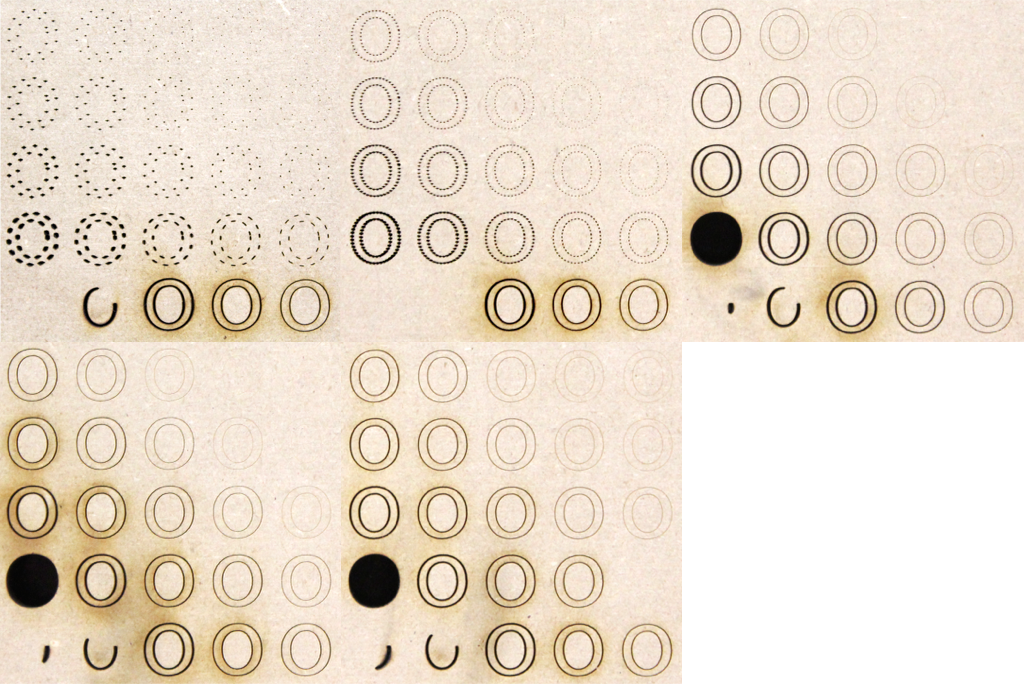
\includegraphics[width=0.4\textwidth]{figures/engravings}
  \caption{%
    A user of the laser cutter has to manipulate the laser's parameters to get the desired appearance.
    Black holes are when the laser passes completely through the material---
    the center is cut out and falls through.
  }\label{fig:rasters}
\end{figure}

\andrew{Make sure to tie this into what my contributions are to our class and what they should take away.}

As you enter the Invention Lab, Berkeley's student hackerspace, you quickly notice that learning to work with fabrication machines is hard.
Scorched cardboard sits atop the scrap pile from laser-cut materials that caught fire.
Failed 3D prints line the foyer walls, deformed from thin supports and improper orientations.
Consider what it takes to configure a laser cutter to ``raster'' images onto workpieces:
four different parameters control the depth, speed, and fidelity of the image etched into the material.
Improper values cause the image to appear only faintly, or melt the material (see Figure~\ref{fig:rasters}).

This research pursues a vision for fabrication machines that help users learn how to operate them.
My key insight is that a fabrication machine can be equipped with an active learning algorithm to enable mixed initiative exploration of a parameter space.
I implement this for a laser cutter and a maker rastering images.
My intended contributions are:
\begin{enumerate}
\item A catalog of user problems realizing design intent with laser cutters
\item Application of active learning to discovering an ideal fabrication machine configuration
\item A comparison of mixed initiative parameter exploration with self-led approaches
\end{enumerate}

To understand frequency, severity, and types of errors makers encounter with laser cutters, I will interview a small number of student members of the Invention Lab.

I will implement an active learning algorithm~\cite{settles_active_2010} to guide a machine, with a user's help, to some subjective ideal configuration for rastering an image.
Each configuration will comprise laser power, speed, frequency, and resolution.
The algorithm will suggest configurations and demonstrate them by rastering an image.
The algorithm will collect a user's rating of raster quality.
As the learned model will predict an continuous value, I will draw from past work for actively learning continuous-value models (e.g.~\cite{sugiyama_active_2008}).
% Currently, I suspect that a Gaussian kernel function or a quadratic curve will best express a user's perception of the quality of a configuration in actualizing their design.

To understand the trade-offs of this method of mixed initiative parameter space exploration, I will run a usability study.
Participants will be asked to recover a configuration for rastering an image that matches an exemplar I provide.
The method of parameter exploration will be varied:
in one condition, participants explore configurations on their own.
In the other, participants explore the configuration space prompted by the examples provided by the active learning algorithm.
Among other metrics, I will measure the total number of configurations tested, and Likert scale and open-ended feedback on perceptions of the experience.

The usability study will use a Universal Laser Systems VLS3.50 machine.
I have received clearance to work with this equipment.
Given the limited time available for the hardware, the proposed usability study will likely include around 4--6 participants.


\section{Conclusion}

People frequently have to work with machines to achieve some subjective goal with parameters they do not understand.
This paper compares two algorithms to help humans achieve such goals by systematically exploring parameter spaces.
While the Nelder-Mead optimization method appears less random to users than Bayesian optimization, the latter appears less likely to prematurely converge.
Future work should address three issues.
First, it should provide a systematic review of algorithms equipped to solve this problem and a comparison of human perceptions of these methods.
Second, it should explore a wider range of mechanisms for expressing rankings, beyond just pairs and sorted lists.
Third, it should do this in a domain-independent way, beyond just fabrication machines.


\section{Acknowledgments}

Acknowledgments.

% Balancing columns in a ref list is a bit of a pain because you
% either use a hack like flushend or balance, or manually insert
% a column break.  http://www.tex.ac.uk/cgi-bin/texfaq2html?label=balance
% multicols doesn't work because we're already in two-column mode,
% and flushend isn't awesome, so I choose balance.  See this
% for more info: http://cs.brown.edu/system/software/latex/doc/balance.pdf
%
% Note that in a perfect world balance wants to be in the first
% column of the last page.
%
% If balance doesn't work for you, you can remove that and
% hard-code a column break into the bbl file right before you
% submit:
%
% http://stackoverflow.com/questions/2149854/how-to-manually-equalize-columns-
% in-an-ieee-paper-if-using-bibtex
%
% Or, just remove \balance and give up on balancing the last page.
%
\balance{}

% REFERENCES FORMAT
% References must be the same font size as other body text.
\bibliographystyle{SIGCHI-Reference-Format}
\bibliography{references}

\end{document}

%%% Local Variables:
%%% mode: latex
%%% TeX-master: t
%%% End:
